% Generated by empirical_bloomberg_20261030/make_empirical_section.py from frozen Bloomberg inputs.
% Main cohort: VIX, OVX, MOVE, BTC DVOL, ETH DVOL. Legacy ATM series remain in the package notes.
\subsection{Data}
\label{sec:empirical-data}
% [AI-DRAFT BEGIN: data paragraph, 30 Oct 2026. Author pass pending.]
The primary histories are Bloomberg \texttt{PX\_LAST} closes of the VIX, OVX and
MOVE indices from 1 January 2000 to 28 October 2026, the last completed US session
before acquisition.\footnote{Fetched on 29 October 2026 with the \texttt{bbg-fetch}
package (BloombergFetch 3.2.2, \url{https://github.com/ArturSepp/BloombergFetch}).
The request, identifiers, adjustment flags and file checksums are recorded in the
replication package. Bloomberg inputs are licensed and are not redistributed.}
VIX and OVX are divided by 100 into decimal annualised price volatility. MOVE is
kept in annualised yield-volatility basis points, because it is a normal
volatility of Treasury yields and not a price volatility. The reference series are
the SPX index, the USO exchange-traded fund (ETF) and the ten-year constant-maturity yield, with price
returns in logarithms and yield changes in basis points. Table~\ref{tab:empirical-data}
gives the coverage.
The primary cohort also includes BTC and ETH DVOL, Deribit's option-based indices
targeting 30-day annualised volatility, from 24 March 2021 to 28 October 2026
(2,045 calendar-day observations each).\footnote{Daily open, high, low and close observations from
\url{https://docs.deribit.com/api-reference/market-data/public-get_volatility_index_data}.
Methodology: \url{https://insights.deribit.com/exchange-updates/dvol-deribit-implied-volatility-index/}.
Native index points are divided by 100. The daily timestamp labels the start of
the candle, so its close is paired with the USD spot index at next-date 00:00 UTC.
Exact timestamps, raw responses and checksums are retained.}
The DVOL observation windows contain weekends,
whereas the Bloomberg series use reported sessions, and the common 30-day target
does not make the index constructions identical.
The replication package documents the remaining conventions (adjustment flags, gap
rules, source reconciliation), plots the five index histories, and reports the earlier
Deribit ATM series for BTC and ETH, whose tenor metadata cannot be verified and which
we therefore keep out of the main comparison.
% [AI-DRAFT END]

\begin{table}[htbp]\centering\small\setlength{\tabcolsep}{4pt}
\begin{tabular}{@{}l P{39mm} r P{31mm} r@{}}\toprule Series & Sample & $N$ & Native mean (interval) & Common mean\\\midrule

VIX & 2000-01-03 to 2026-10-28 & 6779 & 19.8 [17.7, 22.3] & 19.0 \\

OVX & 2007-05-10 to 2026-10-28 & 4903 & 39.3 [35.1, 43.4] & 42.1 \\

MOVE & 2000-01-03 to 2026-10-28 & 6906 & 89.2 [80.2, 99.6] & 97.5 \\

BTC DVOL & 2021-03-24 to 2026-10-28 & 2045 & 59.5 [50.7, 71.3] & 59.6 \\

ETH DVOL & 2021-03-24 to 2026-10-28 & 2045 & 73.5 [61.8, 83.8] & 73.5 \\

\bottomrule\end{tabular}
\caption{Coverage of the five primary volatility indices. Means are percentage
price volatility, except MOVE (yield-volatility bp). Native-mean brackets are
pointwise 95\% circular-block intervals with 250-observation blocks and 400
resamples under a stationary approximation. Common-date means use 1397 observations from 2021-03-24 to 2026-10-28, the intersection of the five date labels.
These are comparable coverage windows, not synchronous closes. Source: Bloomberg
and Deribit, fetched 29 October 2026.}
\label{tab:empirical-data}\end{table}

\subsection{Observed leverage signs across assets}
\label{sec:empirical-beta}
% [AI-DRAFT BEGIN: leverage-sign findings, 30 Oct 2026. Author pass pending.]
The sign of the return--volatility dependence is asset specific. At a 65-observation span
the trailing regression slope of index changes on reference returns is positive on
0.0\% of VIX days, 17.0\% of OVX days and, against yield changes, on 63.9\% of MOVE days (Table~\ref{tab:empirical-beta} and
Figure~\ref{fig:observed-beta}). Across the fifteen established Cboe indices in
Table~\ref{tab:cboe-panel}, broad equity indices stay below 3\%, while gold
(GVZ, 53.4\%) and the Treasury ETF (VXTLT, 46.3\%) alternate between positive and negative regimes.
These observations motivate specifications capable of reproducing both signs of
observed return--index dependence. Their implications for a latent leverage
coefficient depend on the observation map and inference assumptions of
Section~\ref{sec:observations}.

BTC and ETH DVOL have positive span-65 slopes on \betaPosBTCDVOL\% and
\betaPosETHDVOL\% of fitted days, respectively (lower panels of
Figure~\ref{fig:observed-beta}). Their median slopes remain
negative, and the longer-span estimates spend less time above zero. Thus the
crypto indices add examples of changing dependence and do not show a universally
positive crypto leverage effect. The pointwise-band and sign-frequency columns
in Table~\ref{tab:empirical-beta} distinguish a positive fitted slope from one
whose pointwise interval excludes zero.

We estimate $\Delta I_t=a_t+b_t x_t+e_t$ by trailing exponentially weighted least
squares with an intercept, at spans of 65 and 260 observations and a five-span
window, where $x_t$ is the log return of the reference asset (the yield change in
basis points for MOVE). For MOVE a positive slope therefore means that yield
volatility rises with yields, which is the convention of a rate model and the
opposite of the bond-price convention used for VXTLT. Each estimate uses
observations through the fitted date.
Pointwise bands use weighted Newey--West covariance with five lags, and
sign-frequency intervals resample the fitted sign indicators in blocks equal to
the span. These are slopes of an observed index on an observed return. By the
observation map of Section~\ref{sec:observations} they are not the latent
coefficient $\beta$ and are not inserted into the condition $C_Q-\beta\geq0$.
% [AI-DRAFT END]

\begin{table}[htbp]\centering\small\begin{tabular}{@{}l r r r r@{}}\toprule Series & Span & Estimates & Positive (\%, interval) & Lower band $>0$ (\%)\\\midrule

VIX & 65 & 6678 & 0.0 & 0.0 \\

VIX & 260 & 6483 & 0.0 & 0.0 \\

OVX & 65 & 4833 & 17.0 [10.6, 23.0] & 5.2 \\

OVX & 260 & 4638 & 10.2 [0.9, 22.6] & 3.6 \\

MOVE & 65 & 6838 & 63.9 [56.3, 71.5] & 32.9 \\

MOVE & 260 & 6643 & 69.9 [55.9, 82.7] & 36.7 \\

BTC DVOL & 65 & 1980 & 34.8 [21.1, 49.0] & 14.5 \\

BTC DVOL & 260 & 1785 & 19.2 [0.0, 42.0] & 5.4 \\

ETH DVOL & 65 & 1980 & 30.4 [17.5, 42.9] & 7.0 \\

ETH DVOL & 260 & 1785 & 14.4 [0.0, 34.5] & 0.3 \\

\bottomrule\end{tabular}\caption{Share of days with a positive observed volatility beta.
Intervals are conditional block-bootstrap intervals of the fitted sign indicator, and a
constant indicator (VIX) has no interval. The last column is the share of days on
which the lower Newey--West band excludes zero. MOVE uses a yield-change regressor in
different units. DVOL spans count calendar days and Bloomberg spans count retained
sessions. Sources: Bloomberg and Deribit, with coverage in Table~\ref{tab:empirical-data}.}\label{tab:empirical-beta}\end{table}

\begin{figure}[tbp]\centering
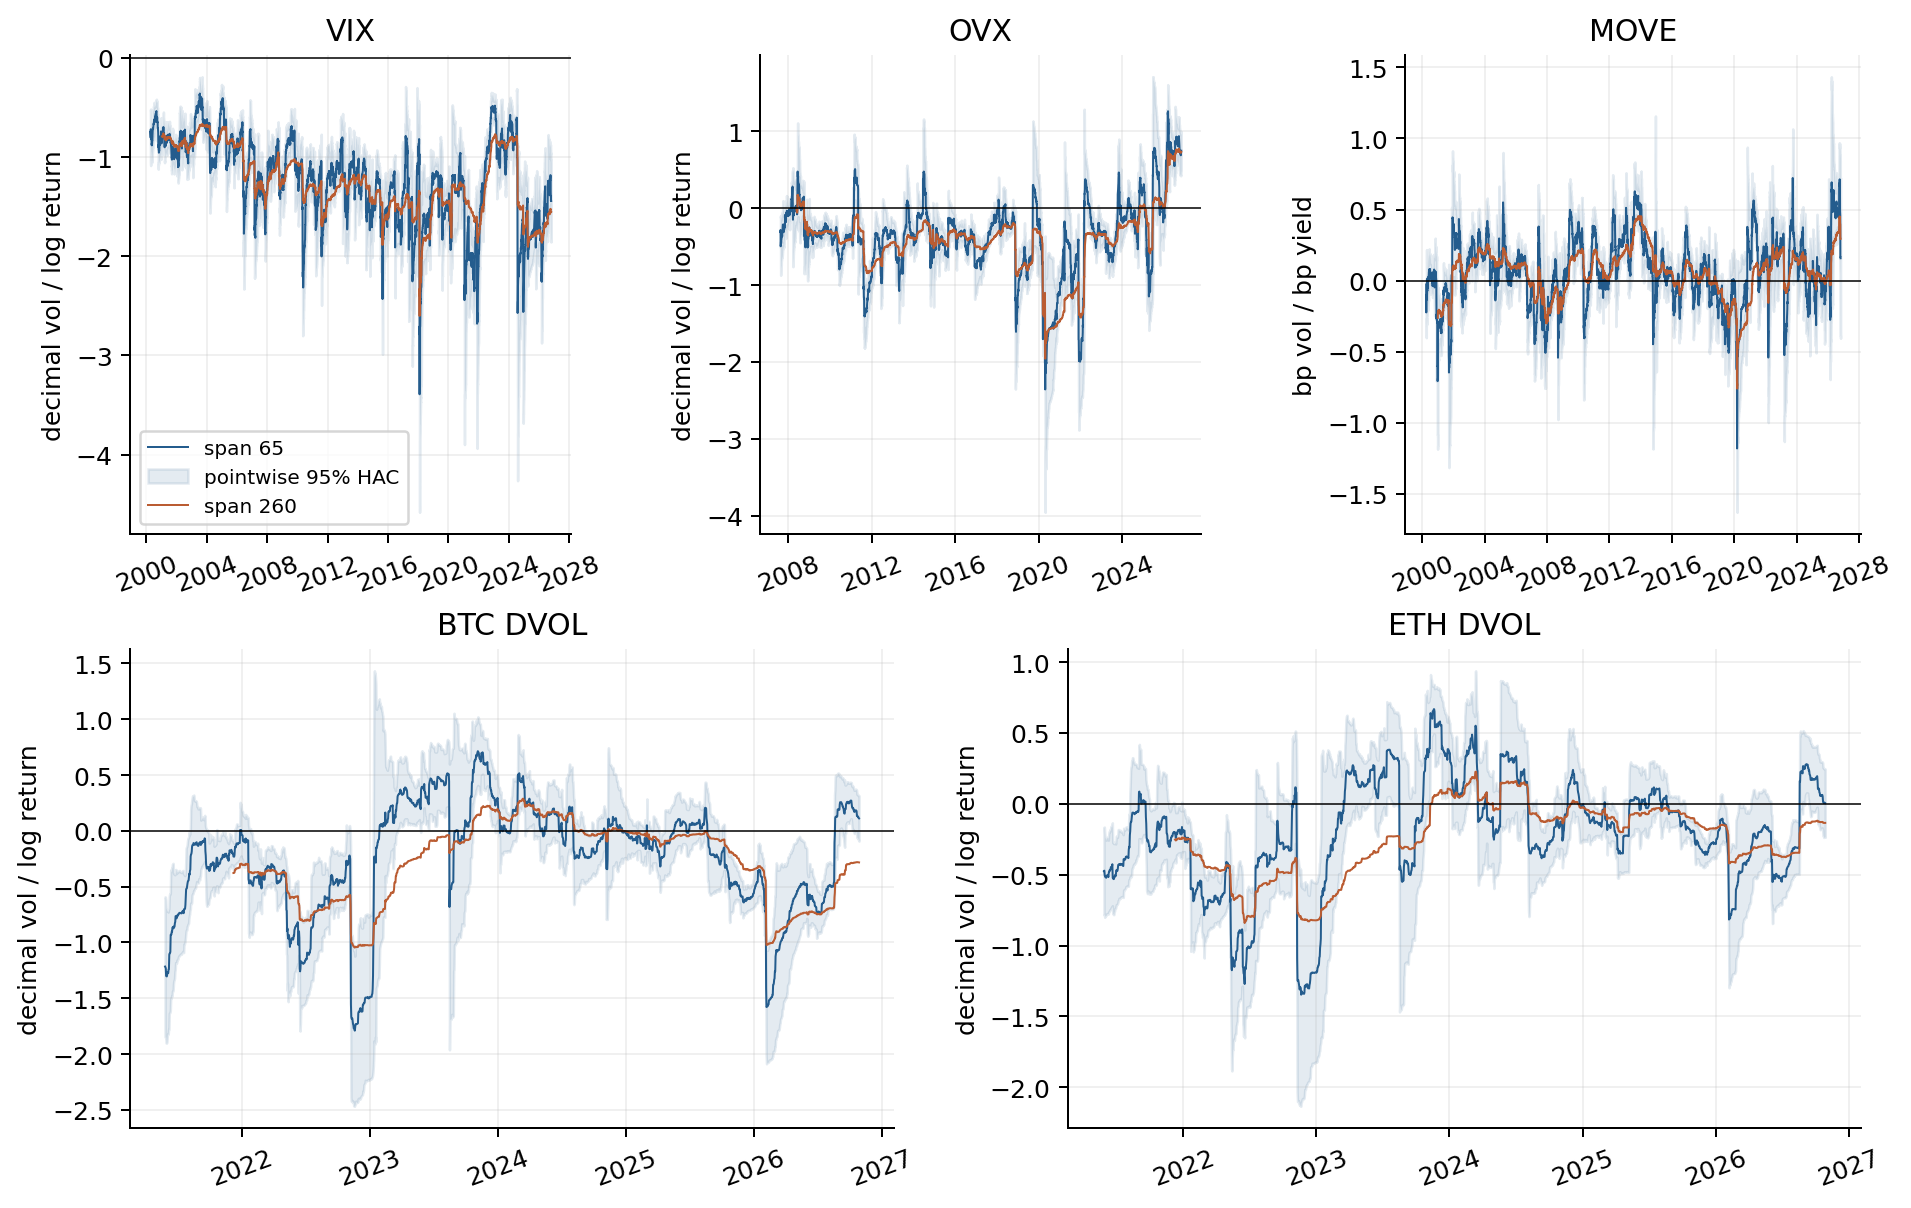
\includegraphics[width=\textwidth,height=.55\textheight,keepaspectratio]{figures/empirical_bloomberg_20261030/beta_five.png}
\caption{Observed level-beta paths for VIX, OVX and MOVE (top) and for BTC and ETH DVOL (bottom). Blue: span 65 with pointwise 95\% Newey--West bands. Orange: span 260. MOVE is bp of yield volatility per bp of yield change, and the other slopes are decimal volatility per log return. Bloomberg spans count retained sessions, DVOL spans count calendar days, and DVOL dates label the candle start. Sources: Bloomberg, 2000--2026, and Deribit, 24 March 2021 to 28 October 2026.}\label{fig:observed-beta}\end{figure}

% [AI-DRAFT BEGIN: Cboe panel paragraph, condensed from the 29 Oct draft.]
Cboe's named volatility indices extend the comparison to fifteen established
price-volatility histories with a common 30-day target, selected from the index
methodology before any outcome was examined.\footnote{Cboe Selected Broad-Based
Index, Equity and ETF Volatility Indices, version 9.0, 30 March 2026:
\url{https://cdn.cboe.com/api/global/us_indices/governance/Volatility_Index_Methodology_Selected_Broad_Based_Index_Equity_and_ETF_Volatility_Indices.pdf}.
Newer and relaunched candidates are inventoried in the replication package and are not pooled.}
Native histories can contain pre-launch calculated values, so Table~\ref{tab:cboe-panel}
also reports the common post-launch sample of 2898 sessions from 2015-04-22 to 2026-10-28.
Single-stock indices add firm-specific variation that a daily panel does not
isolate, and correlated markets share shocks, so the fifteen series are not
fifteen independent replications. The table also carries the held-out GIG-minus-Heston
log scores of Section~\ref{sec:empirical-density} on the native histories. The
common-session scores and the span-260 fractions are in the replication package.
% [AI-DRAFT END]

{\small\setlength{\tabcolsep}{3pt}\begin{longtable}{@{}l P{22mm} l r r r r r l@{}}\caption{Established Cboe volatility-index panel. Positive-beta columns are percentages of days at span 65 on the native history and on the common post-launch sessions. ACF$_{63}$ is the lag-63 level correlation. Score is the held-out GIG minus Heston-marginal mean log score on the native history, with its pointwise 95\% circular-block interval (65 observations), from a chronological 70/30 split per series with the training fit held fixed. The intervals come from a separate resampling run with its own seed, so the VIX and OVX intervals differ by resampling error from those of Table~\ref{tab:empirical-scores}. Source: Bloomberg, with all histories ending on 28 October 2026.}\label{tab:cboe-panel}\\\toprule Index & Reference & First value & $N$ & Native $+$ & Common $+$ & ACF$_{63}$ & Score & 95\% interval\\\midrule\endfirsthead\toprule Index & Reference & First value & $N$ & Native $+$ & Common $+$ & ACF$_{63}$ & Score & 95\% interval\\\midrule\endhead

VIX & SPX & 2000-01-03 & 6779 & 0.0 & 0.0 & 0.521 & 0.163 & [0.053, 0.287] \\

OVX & USO & 2007-05-10 & 4903 & 17.0 & 21.4 & 0.307 & 0.083 & [-0.023, 0.192] \\

RVX & RTY & 2004-01-02 & 5740 & 0.1 & 0.2 & 0.541 & 0.059 & [-0.046, 0.180] \\

VXN & NDX & 2001-02-02 & 6475 & 0.0 & 0.0 & 0.707 & 0.135 & [0.052, 0.218] \\

VXD & INDU & 2000-01-03 & 6750 & 0.7 & 1.8 & 0.527 & 0.169 & [0.062, 0.295] \\

GVZ & GLD & 2008-06-03 & 4634 & 53.4 & 66.4 & 0.600 & 0.136 & [0.047, 0.209] \\

VXEEM & EEM & 2011-03-16 & 3929 & 2.1 & 2.9 & 0.317 & 0.113 & [0.028, 0.184] \\

VXEFA & EFA & 2008-01-02 & 4736 & 0.7 & 0.9 & 0.517 & 0.234 & [0.150, 0.310] \\

VXEWZ & EWZ & 2011-03-16 & 3929 & 2.4 & 0.9 & 0.323 & 0.153 & [0.079, 0.216] \\

VXTLT & TLT & 2004-01-02 & 5733 & 46.3 & 43.1 & 0.578 & 0.043 & [-0.123, 0.352] \\

VXAPL & AAPL & 2011-01-07 & 3975 & 4.3 & 0.8 & 0.361 & 0.072 & [0.012, 0.131] \\

VXAZN & AMZN & 2011-01-07 & 3975 & 12.8 & 7.6 & 0.540 & -0.002 & [-0.020, 0.016] \\

VXGOG & GOOG & 2011-01-07 & 3975 & 7.5 & 8.2 & 0.531 & -0.072 & [-0.126, -0.012] \\

VXGS & GS & 2011-01-07 & 3975 & 0.9 & 1.2 & 0.393 & 0.087 & [0.011, 0.176] \\

VXIBM & IBM & 2011-01-07 & 3975 & 21.5 & 24.5 & 0.570 & 0.080 & [-0.028, 0.233] \\

\bottomrule\end{longtable}}

\subsection{Stationary marginals and chronological transfer}
\label{sec:empirical-density}
% [AI-DRAFT BEGIN: marginal-fit findings with the 3/2 family, 30 Oct 2026. Author pass pending.]
Marginal transfer depends on the asset and the evaluation period. VIX favours the
GIG family over the Heston marginal with an interval above zero, OVX favours it as
a point estimate, MOVE does not, and DVOL separates the two heavy-tailed families.
We fit four stationary
families to the first 70\% of each history by maximum likelihood and evaluate the
mean log score on the last 30\%: the GIG law in volatility, including its exact
Gamma and inverse-Gamma limits, the Heston marginal $2s\,p_V(s^2)$ with $V$ Gamma,
the 3/2 marginal $2s\,p_V(s^2)$ with $V$ inverse-Gamma, and the lognormal law.
Table~\ref{tab:empirical-scores} reports the held-out differences in favour of the
GIG candidate. Against the Heston marginal the VIX difference is 0.163 with
a block interval above zero, and the score column of Table~\ref{tab:cboe-panel}
is positive for 13 of 15 indices, with 9 intervals above zero and 1 below. Against the 3/2 marginal the VIX difference is -0.009, with an
interval that contains zero, so the two power-tailed laws are indistinguishable on
this criterion. Figure~\ref{fig:observed-density} shows the fitted survival
functions against the held-out Bloomberg tails.

The two DVOL training fits select interior GIG laws. On BTC DVOL, GIG-minus-Heston
and GIG-minus-3/2 scores are \scoreBTCDVOLHeston\ and \scoreBTCDVOLThreeHalf,
with both intervals including zero. On ETH DVOL, the corresponding differences are
\scoreETHDVOLHeston\ and \scoreETHDVOLThreeHalf, and both intervals exclude zero, so
ETH DVOL favours GIG against Heston and the 3/2 marginal against GIG. ETH also favours the
lognormal law over GIG. Thus there is no common winning marginal family across
the five indices. Both crypto evaluation samples have no observation above their
own training 95th percentile, so this is transfer to a lower-volatility period
and not a stress-tail validation. DVOL survival plots and persistence diagnostics are
in the replication package.

The fitted GIG law selects its inverse-Gamma limit, the boundary $C=0$ of
Proposition~\ref{prop:stationary}, for VIX and OVX, and an
interior law for MOVE, BTC DVOL, ETH DVOL. An index marginal is the law of
$F(\sigma)$ rather than of $\sigma$, so the VIX and OVX fits do not estimate the latent
physical drift. The index fits motivate examining the inverse-Gamma boundary,
without identifying $C_P=0$ for latent volatility. If a separately estimated latent
physical model has $C_P=0$, then~\eqref{eq:pq-map} gives
$C_Q=\beta\ell_0+\varepsilon\ell_1$. A valid pricing density and stock martingality
jointly require the projected risk price to satisfy
$\beta\ell_0+\varepsilon\ell_1\geq\max(\beta,0)$.
For $\beta>0$, this requires a positive quadratic coefficient under the pricing
measure, although $C_Q\geq\beta$ need not hold with equality. This conditional
model construction is distinct from an inference about latent dynamics from
the index marginals.

For a fitted inverse-Gamma index law with shape $\alpha>0$, positive moments of
order $r$ are finite if and only if $r<\alpha$, and diverge for $r\geq\alpha$.
The fitted shapes are about 8 for both series, so the fitted index laws have finite
moments up to order seven and divergent moments above order eight.

These are comparisons of marginal families on an observed index, not of calibrated
dynamic models. Normalisation uses the training median only, score intervals hold
the training fit fixed, and the single chronological split is descriptive.
% [AI-DRAFT END]

\begin{table}[htbp]\centering\small\setlength{\tabcolsep}{3pt}\begin{tabular}{@{}l P{24mm} P{36mm} P{36mm} P{36mm}@{}}\toprule Series & GIG law & GIG minus Heston & GIG minus 3/2 & GIG minus lognormal\\\midrule

VIX & Inverse-Gamma & 0.163 [0.049, 0.269] & -0.009 [-0.036, 0.013] & 0.028 [-0.001, 0.059] \\

OVX & Inverse-Gamma & 0.083 [-0.022, 0.183] & 0.027 [0.006, 0.051] & -0.005 [-0.034, 0.023] \\

MOVE & Interior GIG & -0.035 [-0.115, 0.045] & 0.043 [0.010, 0.077] & -0.026 [-0.054, -0.000] \\

BTC DVOL & Interior GIG & 0.028 [-0.044, 0.097] & 0.036 [-0.048, 0.128] & 0.007 [0.002, 0.012] \\

ETH DVOL & Interior GIG & 0.081 [0.059, 0.105] & -0.093 [-0.167, -0.021] & -0.036 [-0.050, -0.024] \\

\bottomrule\end{tabular}\caption{Held-out mean log-score differences in favour of the selected GIG candidate, with pointwise 95\% circular-block intervals (65 observations, 400 resamples). Heston denotes the square-root-Gamma marginal and 3/2 the square-root-inverse-Gamma marginal. Training on the first 70\% of each history, evaluation on the last 30\%. Sources: Bloomberg and Deribit, with coverage in Table~\ref{tab:empirical-data}.}\label{tab:empirical-scores}\end{table}

\begin{figure}[tbp]\centering
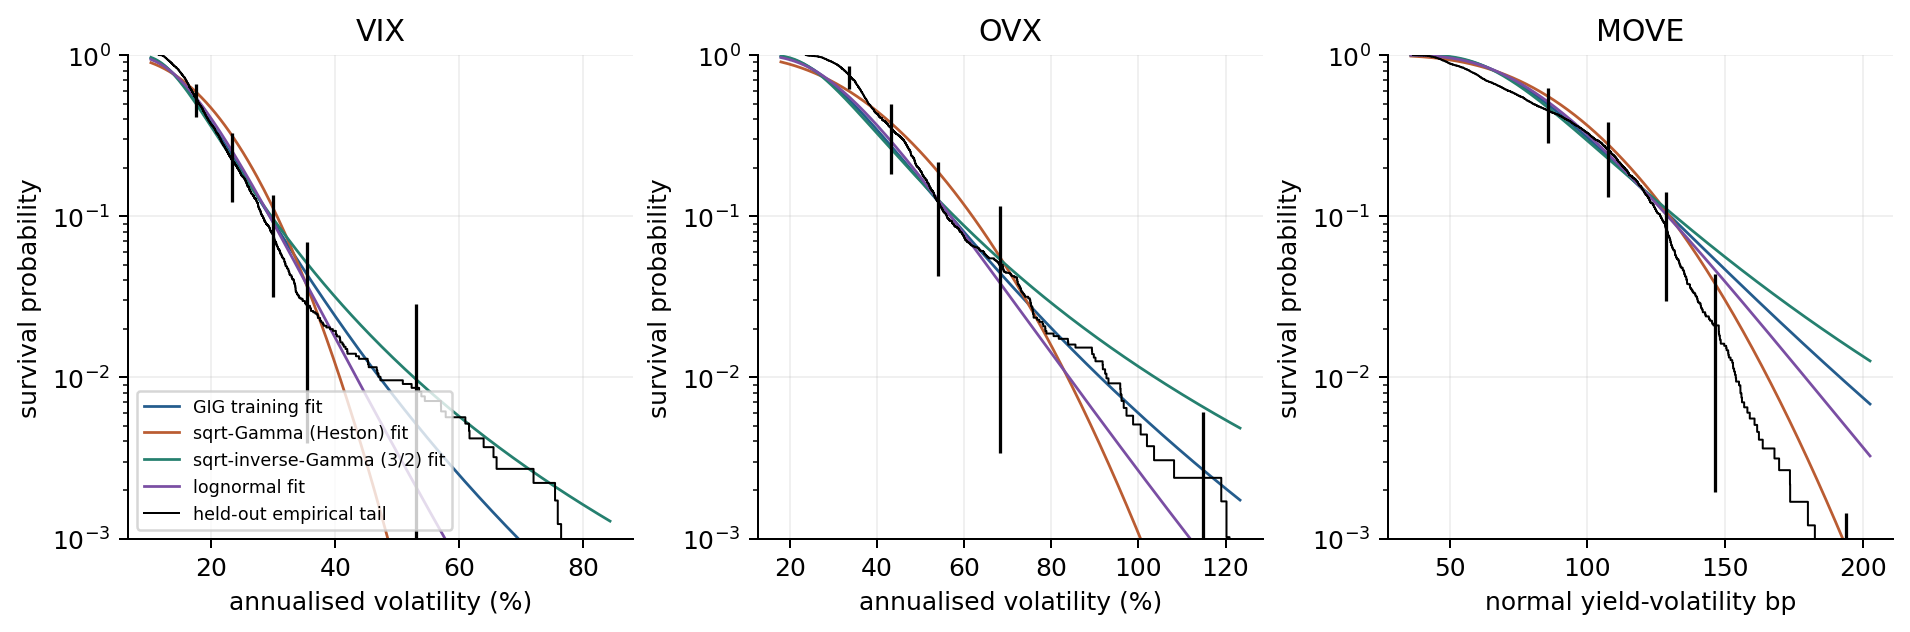
\includegraphics[width=\textwidth,height=.4\textheight,keepaspectratio]{figures/empirical_bloomberg_20261030/density_main.png}
\caption{Training-fitted survival functions and held-out empirical tails for VIX, OVX and MOVE. Bars are pointwise block intervals at training quantiles, and the logarithmic axis is truncated below 0.001. Source: Bloomberg, 2000--2026.}\label{fig:observed-density}\end{figure}

\subsection{Observed persistence}
\label{sec:empirical-acf}
% [AI-DRAFT BEGIN: persistence paragraph, condensed. Author pass pending.]
Lag correlations of the index levels decay slowly and unevenly across assets.
At lag 120 the correlations are VIX: 0.363, OVX: 0.196, MOVE: 0.649, BTC DVOL: 0.703, ETH DVOL: 0.600, and the lag-63 values of the Cboe panel in
Table~\ref{tab:cboe-panel} range from 0.31 (OVX) to 0.71 (VXN). We compute Pearson correlations of lagged level pairs at lags 1 to 120
observations, with circular blocks of 250 observations resampling the lag-pair
vectors. The correlation paths and their pointwise block intervals are in the
replication package. These diagnostics assume a stationary approximation despite visible regime
changes. They do not identify roughness or the latent mean-reversion clock, for the
two reasons developed in Section~\ref{sec:observations}: the observable is a map of
the state, and finite samples can bias an ACF estimator. The synthetic study below
illustrates this bias using a full-sample-centred estimator. Its centring and
variance normalisation differ from the lag-pair Pearson estimator used here,
so its bias values do not quantify the bias of these empirical estimates.
% [AI-DRAFT END]

\subsection{Synthetic observation maps and finite-sample persistence}
\label{sec:synthetic-observation-acf}
% [AI-DRAFT BEGIN: updated VIX calibration and synthetic results. Author pass pending.]
We fit the quadratic-drift model to 6,779 daily Bloomberg VIX closes
from January 2000 through October 2026 (Table~\ref{tab:empirical-data}).
For each pair $(\kappa_1,\kappa_2)$, we choose $\theta$ and total volatility of volatility $v$
by matching the stationary log-volatility density to a 50-bin histogram of $\log(\mathrm{VIX}/100)$.
We then choose $(\kappa_1,\kappa_2)$ by matching daily VIX level
autocorrelations at lags 1 to 119. Both steps minimise sums of squared errors.
For each pair we average the model autocorrelations over 10,000 ten-year paths with common random shocks.
The fitted index coefficients are $(\theta,\kappa_1,\kappa_2,v)=(0.1995,0.2000,9.1829,0.6851)$.
The estimate of $\kappa_1$ reaches its lower search bound of $0.2$.

We use these coefficients for the latent state in a synthetic observation experiment.
The two Brownian loadings enter the index dynamics only through $v^2=\beta^2+\varepsilon^2$. We choose $\beta=0.35$
for illustration and set the residual loading to $\sqrt{v^2-\beta^2}$.
We set $Q=P$ to isolate the observation map $F_\tau(\sigma)$, the ideal
variance-swap volatility at $\tau=30/365$ years.

The stationary mean and standard deviation are 0.17967
and 0.06326 for latent volatility and 0.18125 and
0.05856 for the mapped index. At the stationary median
$\sigma=0.17142$, the map gives $F_\tau(\sigma)=0.17479$.
The instantaneous index-level beta is $\beta F_\tau'(\sigma)=0.33076$.
The 30-day observation horizon thus changes both the stationary distribution
and the return sensitivity even when $Q=P$.
% [AI-DRAFT END]

We multiply $(\kappa_1,\kappa_2,v^2)$ by clocks $c=1$ and $c=0.25$,
holding $\theta$ fixed and multiplying $\beta$ by $\sqrt{c}$.
This preserves the latent invariant distribution while replacing its
population autocorrelation $\rho(h)$ by $\rho(ch)$.
We recompute the fixed-maturity observation map for each clock.
For each regime, 400 independent paths start from the invariant GIG distribution.
We record 252 observations per model year with four positive splitting steps per observation.
The sample ACF uses the full-sample mean. At lag $h$ we divide the cross-product
sum by $N-h$ and the sum of squared deviations by $N$.
Table~\ref{tab:synthetic-acf-bias} reports the bias at lag 63.
Figure~\ref{fig:synthetic-acf-bias} shows its lag profile.

\begin{table}[htbp]\centering\small
\begin{tabular}{rrrrrr}\toprule
Clock & Years & Population ACF & Mean sample ACF & Bias & MC s.e.\\
\midrule

1.00 & 5 & 0.5991 & 0.4481 & -0.1509 & 0.0080 \\

1.00 & 10 & 0.5991 & 0.5260 & -0.0731 & 0.0061 \\

1.00 & 20 & 0.5991 & 0.5698 & -0.0293 & 0.0041 \\

0.25 & 5 & 0.8767 & 0.6366 & -0.2402 & 0.0088 \\

0.25 & 10 & 0.8767 & 0.7560 & -0.1207 & 0.0057 \\

0.25 & 20 & 0.8767 & 0.8224 & -0.0543 & 0.0034 \\

\bottomrule\end{tabular}
\caption{Synthetic sample-ACF bias at lag 63. Monte Carlo standard errors describe
the estimated mean across independent paths. The three horizons use nested prefixes of each path.}
\label{tab:synthetic-acf-bias}\end{table}

\begin{figure}[htbp]\centering
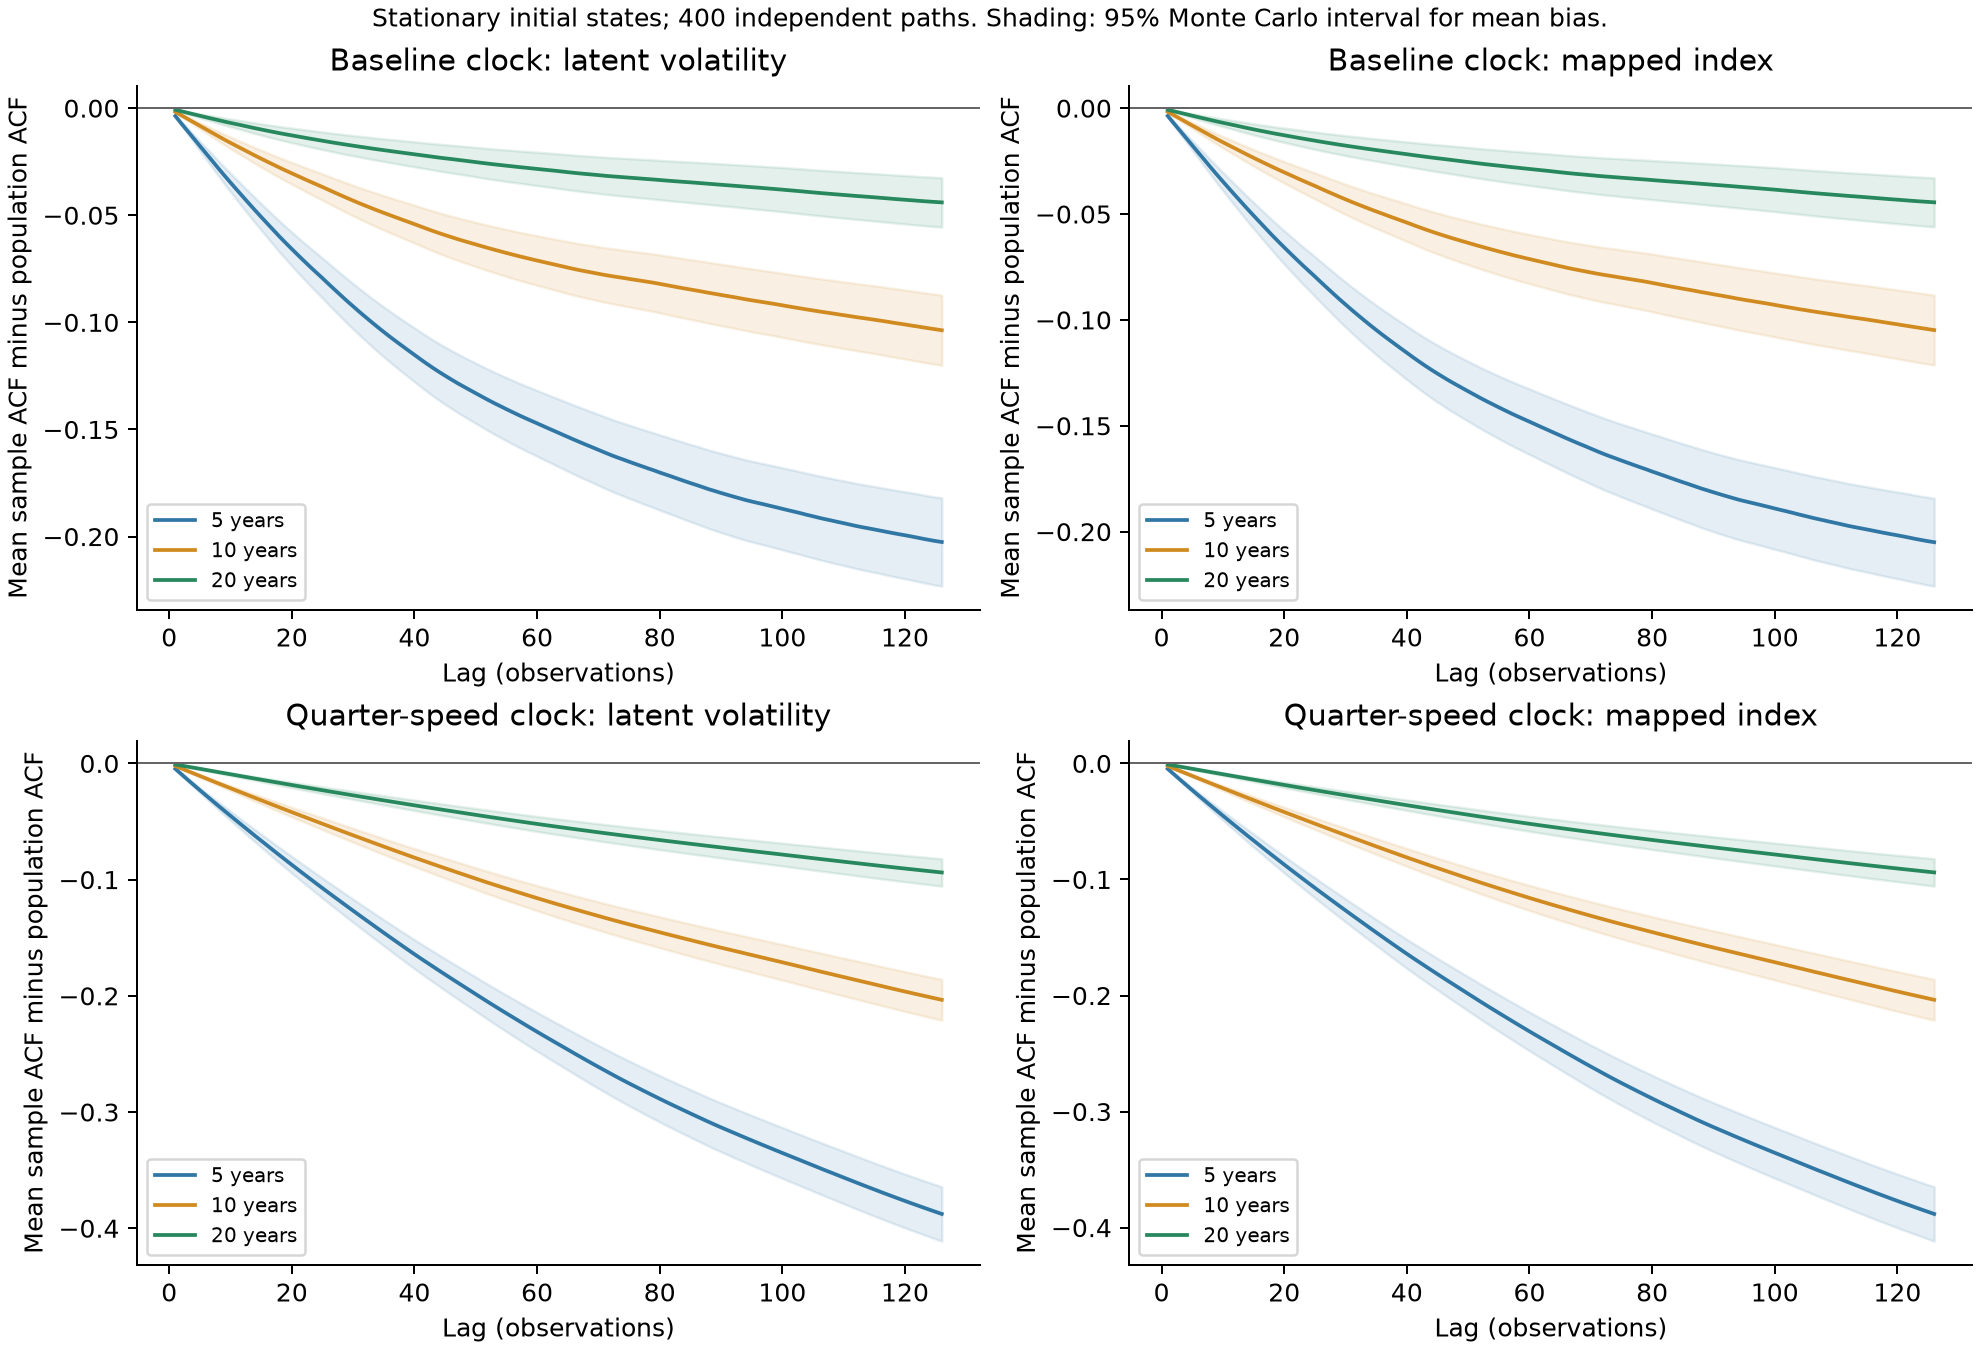
\includegraphics[width=\textwidth,height=.76\textheight,keepaspectratio]{figures/vix_fit_20261123/synthetic_sample_acf_bias.png}
\caption{Average sample-ACF bias for latent and mapped volatility under the two clocks. Shading gives 95\% Monte Carlo intervals for the mean bias.}\label{fig:synthetic-acf-bias}\end{figure}

We compute the observation map and population ACF with a reversible
finite-volume generator on a log-volatility grid. When we double the daily splitting steps
from four to eight, the largest absolute change in the mean latent sample ACF is approximately
$7.5\times 10^{-6}$ across lags 0 to 126.
The replication package also reports grid refinement and independent Monte Carlo checks.

\subsection{Reproducibility and scope}
% [AI-DRAFT BEGIN: scope paragraph, condensed. Author pass pending.]
The replication package\footnote{\url{https://github.com/ArturSepp/StochVolModels},
directory \path{papers/robust_volatility_models_2026/replication}. Code, the Cboe-index pipeline,
quote hashes and every fitted parameter are included. Bloomberg and ThetaData
inputs are licensed and are not included.} stores the inputs, seeds,
results and figures of this section, the synthetic study, and the option-surface
calibrations of Section~\ref{sec:oca-calibration}. The single chronological split
is descriptive, and the block intervals describe sampling error under a stationary
approximation. Joint estimation of latent dynamics from realised and implied
volatility is a separate project.
% [AI-DRAFT END]
